% --------------------------------------------------------------------
% Inclues
% --------------------------------------------------------------------
\documentclass[a4paper,11pt]{article}

\usepackage{fullpage}
\usepackage[utf8]{inputenc}
\usepackage[german]{babel}
\usepackage{amsmath}
\usepackage{amssymb}
\usepackage{amsthm}
\usepackage{listings}
\usepackage{mathrsfs}
\usepackage{graphicx}
\usepackage[backend=biber]{biblatex}
\addbibresource{wator.bib}
\usepackage[babel=true]{microtype} % sexy micro typesetting
%\usepackage{hyperref} % create URLs and clickable refs
%\usepackage{titling} % custom titling

% --------------------------------------------------------------------
% Definitions
% --------------------------------------------------------------------
\newcommand{\R}{\ensuremath{\mathbb{R}}}   % reelle Zahlen
\newcommand{\C}{\ensuremath{\mathbb{C}}}   % complexe Zahlen
\newcommand{\N}{\ensuremath{\mathbb{N}}}   % natrürliche Zahlen
\newcommand{\iu}{{i\mkern1mu}}
\newcommand{\norm}[1]{\left\lVert#1\right\rVert_2}

\newcommand{\comment}[1]{\textbf{\textcolor{blue}{#1}}\newline}

%\theoremstyle{plain}
\newtheorem{theorem}{Satz}[section] % reset theorem numbering for each chapter
\newtheorem{lemma}[theorem]{Lemma}
\newtheorem{definition}[theorem]{Definition}
\newtheorem{remark}[theorem]{Bemerkung}
\newtheorem{example}[theorem]{Beispiel}
\theoremstyle{definition}
\renewcommand{\theequation}{\thesection.\arabic{equation}}
\numberwithin{equation}{section}

\newcommand{\HRule}[1]{\rule{\linewidth}{#1}}   % Horizontal rule

\makeatletter                           % Title
\def\printtitle{%                       
    {\centering \@title\par}}
\makeatother                                    

\makeatletter                           % Author
\def\printauthor{%                  
    {\centering \large \@author}}               
\makeatother  

% --------------------------------------------------------------------
% Metadata
% --------------------------------------------------------------------
	\title{ \normalsize \textsc{Biomathematisches Praktikum am PC 2017}    % Subtitle
            \\[2.0cm]                   % 2cm spacing
            \HRule{1pt} \\ [0.5cm]      % Upper rule + 0.5cm spacing
            \LARGE \textbf{\uppercase{Simulation des Wa-Tor Räuber-Beute Modells und Erweiterungen}}    % Title
            \HRule{1pt} \\ [0.5cm]      % Lower rule + 0.5cm spacing
            \normalsize \today          % Todays date
        }

	\author{
	        Sebastian von der Thannen\\
	        Thomas Heitzinger\\
	        \vspace{10mm}
	        \textsc{Technische Universität Wien}\\
	}


\begin{document}
% ------------------------------------------------------------------------------
% Maketitle
% ------------------------------------------------------------------------------
	\thispagestyle{empty}       % Remove page numbering on this page

	\printtitle                 % Print the title data as defined above
	\vfill
	\printauthor                % Print the author data as defined above
	\newpage
	
% --------------------------------------------------------------------
% Contents
% --------------------------------------------------------------------
	\tableofcontents
	\newpage
	
% --------------------------------------------------------------------
% Begin Document
% --------------------------------------------------------------------
	\section{Das klassische Wa-Tor Programm}

	\section{Das stetige Wa-Tor Programm}
	\subsection{Schwarmverhalten}

	\section{Animationen}

	\section{Helmholtz Equation}
	
	\subsection{General}
	
	The Helmholtz equation is a partial differential equation of elliptic type. 
	
	\begin{alignat}{2} \label{eq:helmholtz}
		\nabla^2 u + \kappa^2 u \enspace &&= \enspace 0 \\
		\textnormal{or} \quad \Delta u + \kappa^2 u \enspace &&= \enspace 0 \nonumber
	\end{alignat}
	where $\Delta$ is the Laplace Operator with $ \Delta u := \sum_{i=1}^{d} \frac{\partial^2 u}{\partial x_i^2}$. \newline
	
	\begin{figure}
		\centering
		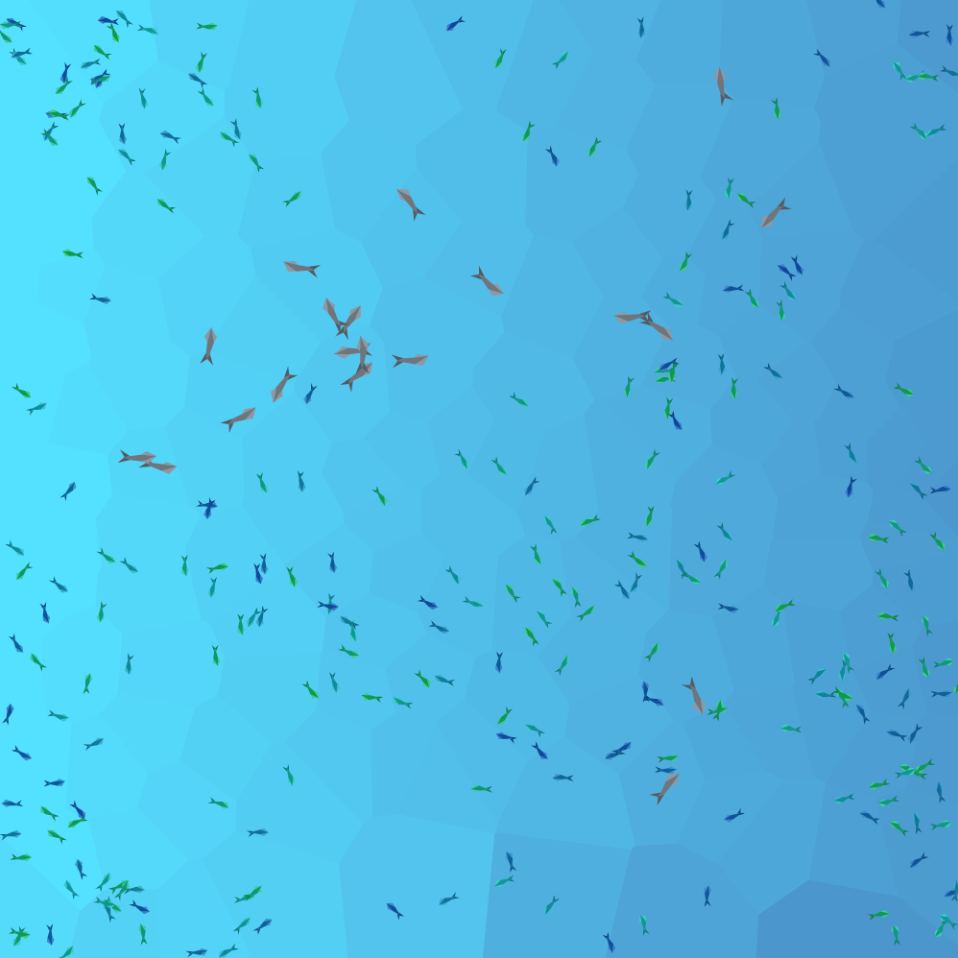
\includegraphics[width=1\textwidth]{pictures/wator.png}
		\label{fig:helmholtz}
		%\caption{Solution to Helmholtz equation}
	\end{figure}
	
	We are interested in radial symmetric solutions to the Helmholtz equation. In order to find them it is helpful to transform equation (\ref{fig:helmholtz}) into polar coordinates for the two dimensional case or spherical coordinates for the three dimensional case. 
	
	\begin{lemma} \label{lemma:laplace}
		The Laplace operator in $\R^2$ is given by $\Delta u = \frac{\partial^2 u}{\partial x^2} + \frac{\partial^2 u}{\partial y^2}$. The Cartesian coordinates can be represented by polar coordinates as follows: 
		\begin{align*}
			\begin{cases}
				x = r \cos \theta \\
				y = r \sin \theta
			\end{cases}
		\end{align*}
		Using these substitutions it can be shown that:
		\begin{align*}
			\Delta u = \frac{\partial^2 u}{\partial r^2} + \frac{1}{r} \frac{\partial u}{\partial r} + \frac{1}{r^2} \frac{\partial^2 u}{\partial \theta^2}
		\end{align*}
		Similarly, in $\R^3$ we transform to a spherical coordinate system:
		\begin{align*}
			\begin{cases}
				x = r \sin \theta \cos \varphi \\
				y = r \sin \theta \sin \varphi \\
				z = r \cos \theta
			\end{cases}
		\end{align*}
		which yields the form:
		\begin{align}
			\Delta u = \frac{1}{r^2} \frac{\partial}{\partial r} \left( r^2 \frac{\partial u}{\partial r} \right) + \frac{1}{r^2 \sin \theta} \frac{\partial}{\partial \theta} \left( \sin \theta \frac{\partial u}{\partial \theta} \right) + \frac{1}{r^2 \sin^2 \theta} \frac{\partial^2 u}{\partial \varphi^2}
		\end{align}
	\end{lemma}
	%\begin{proof}
	%	\comment{probably not interesting enough}
	%\end{proof}
	\vspace{5mm}
	
	Helmholtz' equation is obtained by adding the term $\kappa^2 u$. Since we are solely interested in radial symmetric solutions we would like to eliminate the angular variables $\theta$ and $\varphi$ from the equation. This leads us to:

	
% Figures
	
	\listoffigures
	
% Literatur 


	\nocite{*}
	\printbibliography[heading=bibintoc]% show bibliography in toc
	
\end{document}